\documentclass[]{scrartcl}

\usepackage{graphicx}
\usepackage{multirow}
\usepackage{amsmath}
\usepackage{braket}
\usepackage{graphicx}
\usepackage{subcaption}
\usepackage{rotating}

\usepackage{natbib}

\newcommand{\csqn}{
	\ensuremath{ \chi ^2 / N }}

%opening
\title{PHY 982 - HW 2}
\author{Xingze Mao \\ Zachary Matheson \\ Thomas Redpath}
\date{}

\begin{document}

\maketitle

\section*{Part I: proton and neutron elastic scattering}


In this part, we deal with the elastic scattering of a proton on a target $^{100}$ Mo at two different energies $E_{lab}$=5 and 50 MeV. The reaction code \texttt{fresco} is used to do the calculation and Optical Model Parameter(OMP) is employed. For the proton scattering, we choose the OMP parameters of \citep{Menet1971} for the relevant energies. For the neutron scattering we use the OMPs of \citep{Koning2003}.

1)If no nuclear interaction is included in the scattering, we only have the Coulomb interaction between projectile and target, if the target is treated as a pointlike particle, we will have Rutherford scattering.The differential cross section is

\begin{equation}
\frac{d\sigma}{d\Omega}=\frac{2\pi}{\hbar}\mid M_{fi}\mid^2 D_f
\label{a}
\end{equation}
Here $M_{fi}=\bra{\phi_f}M\ket{\phi_i}$ is the scattering amplitude, $D_f$ is the density of final states.
Using plane wave function, we can get the expression for the scattereing amplitude. When we have pointlike nucleus,
\begin{equation}
M_{fi}=-\frac{Ze^2}{4\pi\epsilon_0}\int\frac{e^{iqR/\hbar}}{|R|}d^3R.  
\end{equation}
Plug this expression into the equation \ref{a}, we can get the angular distribution of Rutherford scattering.If nucleus is of finite size, then 
\begin{equation}
M_{fi}=-\frac{Ze^2}{4\pi\epsilon_0}\int\frac{e^{iqR/\hbar}}{|R|}d^3R\int e^{iqr'/\hbar}\rho(r')d^3r'
\end{equation}

The additional term here is the Fourier transform of the charge distribution, called the form factor. So, if we get the the cross section from experiment, we can obtain the charge distribution of the nucleus by taking the inverse Fourier transformation! 

%In this project, we study the cases of proton and neutron elastic scattering from $ ^{100} \mathrm{Mo} $ using the \texttt{FRESCO} code. Table~\ref{tab:entrance} lists the quantum numbers for the mass partition.

2) Figure~\ref{fig:xsproton} shows the cross sections at energies E=5 MeV and E=50 MeV for neutron and proton elastic scattering. For $E_p=5$ MeV, the ratio is almost 1 in the whole region. For $E_p=50$ MeV shows strong oscilation,whcih means a large deviation from Rutherford scattering. At large distance, the interaction between proton and Mo-100 is dominated by Coulomb repulsion. If the energy of protons is not large enough, they will be reflected and will not come to the point where the strong interaction can have an effect. The scattering pattern will just be the Rutherford scattering cross section. This can be viewed in our results for the two incident proton energies. When we increased the energy to 50 MeV, the nuclear force comes into play and the cross section shows a large deviation from Rutherford scattering. Since there is no Coulomb interaction for the neutron scattering, the angular distributions show a large deviation from Rutherford scattering.

\begin{figure}[!htb]
\centering
\includegraphics[scale=0.5,angle=270]{plots/cs.eps}
\caption{Anuglar distributions for neutron and proton elastic scattering at incident energies of 5MeV and 50MeV.}
\label{fig:xsproton}
\end{figure}


3) To explore the effect of the imaginary part, we first looked at the modulus of the S-matrix for the parameters we have choosen. In Figure~\ref{fig:modpn5} we show the modulus for the partial waves at an incident energy E=5 MeV, and in Figure~\ref{fig:modpn50} for E=50 MeV. In each figure,the points connected by lines are moduli for each partial wave. The boxes at the bottom of each figure are the orbital angular momenta, $L$ divided by 100. Figures~\ref{fig:modpn5} and \ref{fig:modpn50} both show that when we increase the orbital angular momentum, the modulus increases. Higher angular momentum correspondes to a larger potential, since the imaginary part of the optical potential stays the same. We are actually increasing the ratio of real to imaginary part of the optical potential. The imaginary optical potential contributes to the flux leaving the elastic scattering channel. When we decrease the ratio of the imaginary part in the potential, we have less flux leaving and the modulus approaches one. We made an additional test for $E_{\mathrm{inc}}=50$ MeV - see Figure~\ref{fig:modnoimg} - with all imaginary parts of the potential are set to 0. Moduli for all partial waves are found to be 1, showing no flux lost. In Figures~\ref{fig:modpn5} and \ref{fig:modpn50}, many partial waves have the same $L$, although their $J$ values differ by one due to the spin-orbit coupling.

\begin{sidewaysfigure}
	\begin{subfigure}{0.5\textwidth}
		\centering
		\includegraphics[scale=0.4]{plots/05S_module.png}
		\caption{Modules of each partial wave for p(n)+Mo100 at E= 5MeV}
		\label{fig:modpn5}
	\end{subfigure}\quad
	\begin{subfigure}{0.5\textwidth}
	\centering
		\includegraphics[scale=0.4]{plots/50S_module.png}
		\caption{Modules of each partial wave for p(n)+Mo100 at E= 50MeV}
		\label{fig:modpn50}
	\end{subfigure}

	\begin{subfigure}{0.5\textwidth}
	\centering
		\includegraphics[scale=0.4]{plots/i0_S_50_module.png}
		\caption{Modules of each partial wave for p(n)+Mo100 at E= 50MeV with real potential}
		\label{fig:modnoimg}
	\end{subfigure}
\end{sidewaysfigure}


4) Next, we explore the dependence of cross section on nuclear radius. Figure~\ref{fig:radiusp} shows the angular distributions for proton elastic scattering at $50$ MeV for four different nuclear radii. Two trends are apparent in this figure: (1) the compression of the diffraction patterns with increasing size of the scatterer and (2) an increased deviation from Rutherford scattering due to the increased likelihood of nuclear interaction afforded by the larger nucleus. Figure~\ref{fig:radiusn} (neutron elastic scattering) shows similar trends for the diffraction pattern and the total cross section related to the nucleus size (larger nucleaus implies higher likelihood to scatter from it).

10) The total reaction cross section for 5 MeV neutrons is 6100 mb; the absorption cross section is 2700 mb. For 50 MeV neutrons the total reaction cross section is 4200 mb; the absorption cross section is 2100 mb.

\begin{figure}[h]
\centering
	\includegraphics[scale=.5,angle=270]{plots/R_p50fort.eps}
	\caption{cross section for p+Mo100 at E= 50MeV with different radius}
	\label{fig:radiusp}
\end{figure}

\begin{figure}
\centering
	\includegraphics[scale=.5,angle=270]{plots/R_n50fort.eps}
	\caption{cross section for n+Mo100 at E= 50MeV with different radius}
	\label{fig:radiusn}
\end{figure}



%\begin{equation}
%	^{100} \mathrm{Mo} (p,p) ^{100} \mathrm{Mo}
%	\label{eq:therxn}
%\end{equation}

%\begin{equation}
%	^{100} \mathrm{Mo} (n,n) ^{100} \mathrm{Mo}
%	\label{eq:therxn}
%\end{equation}


%\begin{table}
%\centering
%	\begin{tabular}{ | c | c  c | }
%\hline
%	Projectile 1 & $p$ & $ J ^{\pi} = 1/2 ^+ $ \\
%	Projectile 2 & $n$ & $ J ^{\pi} = 1/2 ^+ $ \\
%\hline
%	Target & $ ^{100} \mathrm{Mo} $ & $ J ^{\pi} = 0 ^+ $ \\
%\hline
%	\end{tabular}
%	\caption{Entrance partition's quantum numbers.}
%	\label{tab:entrance}
%\end{table}

%\subsection*{Proton elastic scattering: $E=5,50$ MeV}

%\subsection*{Neutron elastic scattering: $E=5,50$ MeV}


\clearpage
\section*{Part II: Fitting with \texttt{sfresco}}

\subsection*{Real and Imaginary Volume Terms}

To explore \texttt{fresco}'s use for fitting to experimental results (via \texttt{sfresco}), we use the data for $ ^{100} \mathrm{Mo} (p,p)$ at $E_p = 49.4$ MeV from \citep{Sinha1972}. This dataset includes  elastic scattering at three incident energies: $19.85,30.3,49.45$ MeV. We take the $49.45$ MeV data to include in our \texttt{sfresco} input file. These data are in units of mb/sr and span a range in CM angles from 10 to 150 degrees with a quoted error of $\sim 4 \%$. As the starting point for our fit, we take the real and imaginary volume parameters of \citep{Menet1971} for 49MeV incident energy (listed in Table~\ref{tab:init}). We then vary each of the six parameters one at a time to determine which gives the best fit (smallest $\chi ^2 / N$). We then fix this parameter by replacing the value in the potential defined in the \texttt{fresco} input file with this new value found by the fit. We proceed by individually varying the five remaining parameters to again determine which gives the smallest $\chi ^2 / N$, then we input this new value into the \texttt{fresco} input, repeating until all parameters have been fit. Table~\ref{tab:fitvol} reflects the order in which parameters were fit and the $\chi ^2 / N$ values from each fit. The resulting fit compared to the data is shown by the red line in Figure~\ref{fig:fits}.

Next, we use the results from the successive individual fits to initialize a three-parameter fit for the real volumne component. We iterate this three-parameter fit by inputting the results of one run into the initial values of the next until the $\chi ^2 /N$ and the fitted parameters change very little between iterations. We then use these values to update the definition of the real volume component in the \texttt{fresco} input file and repeat the interated three-parameter fit for the imaginary volume component. When this fit has converged, we allow the real volume parameters to vary again to ensure that changes to the imaginary part hasn't perturbed the fit (we noticed only negligible changes to the parameters and $\chi ^2 /N$). The fit results are plotted in Figure~\ref{fig:fits} (green line).

Finally, with the results of the previous step as initial parameters, we perform a six-parameter fit and iterate to arrive at our final fit (the blue line in Figure~\ref{fig:fits}). Table~\ref{tab:fitvol} summarizes the values and $\chi ^2 / N$ at each point in the fitting process; there are only entries for the final values in each step not for each iteration.

\subsection*{Sensitivity to Initialization}

In terms of sensitivity to initialization, we studied the dependence of a multi-iteration, single-parameter fit on the value given as its initial parameter. We began with a potential consisting of real and imaginary volume terms using the six parameters we found in our fit ($\chi ^2 /N = 69$). We then varied the initialization of each parameter to see if, through interating, we could recover the value obtained before. For $V,r_0,a_0,W,r_w$, scaling the initial value by a factor of four in each case caused the fit to converge to an entirely different value with $\chi ^2 /N>100$. For $a_w$, we needed to scale by a factor of $16$ before the fitting routine failed to return the original parameter (with $\chi ^2 /N>100$).

We applied a similar test to a three-parameter fit - changing the initial value for one parameter and seeing how many interations were needed to recover the values of our original fit. For the three real volume parameters, doubling $V,a_0$ required a single iteration to recover the fit values. However, doubling $r_0$ caused \texttt{MINGRAD} to return a ``failed to converge'' message after two iterations. A return to our fit values when two parameters are changed simultaneously depends on which two are changed. Changing $V,a_0$ by a factor of two required one iteration to return. However, changing $r_0$ AND either of the other two resulted in convergence (after three iterations) to completely different values: $12,2.3,0.65$ when $r_0,a_0$ intializations were scaled by 2; when $V,r_0$ intializations were scaled by 2, the fit failed to converge.

Finally, when the initializations for all three parameters are simultaneously doubled, \texttt{MINGRAD} returns a ``terminated without convergence'' error after three iterations. The process described in the previous two paragraphs was carried out for the parameters of the imaginary volume term with similar results. This exercise illustrates the need to have good starting points when fitting data and emphasizes the sensitvity of the fit not only to the initialization but also to the number of parameters being fit.

%For the real and imaginary volume components, $r_0$ is the most sensitive - when its initial value is doubled, the fit converges to a value that is nearly double that reached via the original initialization. In contrast, doubling the initial value for $V$ or $a_0$, the fit recovers the same value reached via the original initialization. In a 3-parameter fit, the $r_0$ and $a_0$ parameters are most sensitive to their initial values - doubling them doubles their fitted values while doubling $V$ results in the same value as was found with its original initialization. From this qualitative investigation, we can conclude that initialization of the parameters in the exponential are most crucial to producing a good fit.

%In the second stage where three parameter fits are used for fine tuning, we found that doubling the initial parameters resulted in non-convergence for the real volume parameters while the imaginary volume parameters were recovered. We attribute this to the fact that there is little change between the imaginary volume parameters listed in the third section of Table~\ref{tab:fitvol} and their counterparts in the the first section.

%Some observations:
%\begin{itemize}
%	\item First derivative depends mainly on interval over which parameter is allowed to vary and step size for next guess
%	\item $\chi ^2 / N$ decreases slightly as each successive parameter is fixed
%	\item Fits are not great: i will try adding the SO to the potential and/or different data
%\end{itemize}


%% INITIAL PARAMETERS %%


\begin{table}
\centering
	\begin{tabular}{ c | c | c c c | c c c | c c c | c c c |  }
	Fit & $E _{\mathrm{in}}$ [MeV] & $ V _0$ & $ r _0$ & $ a _0$ & $W$ & $ r _{w} $ & $ a _{w} $ & $W_s$ &$ r _{ws}$ & $a_{ws}$ & $V_{so}$ & $r_{so}$ & $a_{so}$ \\
\hline
	VOL & 49.0 &  47.0 &  1.16 &  0.75  &  5.6 & 1.37 &  0.51 & & & & & & \\
	SRF & 49.0 &  47.0 &  1.16 &  0.75 & & &  &  4.2 & 1.37 &  0.51 & & & \\
\hline
	SO & 49.0 & 43.8 & 1.16 & 0.77 & 5.5 & 1.36 & 0.42 & & & & 6.0 & 1.06 & 0.78\\
\hline
	\end{tabular}
	\caption{Starting parameters for each component of the fit (from \citep{Menet1971}). VOL refers to fitting with both real and imaginary volume terms. SRF replaces the volume imaginary term with a surface imaginary. SO adds a spin orbit term to the results of the fit using volume real and imaginary terms.}
	\label{tab:init}
\end{table}


%% FIT VOLUME IMAGINARY %%


\begin{table}
\centering
	\begin{tabular}{ c | c | c | c }
	Fit Type & Parameter & Value & $\chi ^2 / N$\\
\hline
	\multirow{6}{*}{Indv. 1-par} & $V$ & 43.8 & 155 \\
	& $W$ & 5.5 & 153 \\
	& $a _w$ & 0.42 & 151\\
	& $a _0$ & 0.77 & 148\\
	& $r _w$ & 1.36 & 144 \\
	& $r _0$ & 1.16 & 144 \\
\hline
	\multirow{3}{*}{3-par} & $V$ & 51.4 & \multirow{3}{*}{124} \\
	& $r_0$ & 1.12 & \\
	& $a_0$ & 0.92 & \\
\hline
	\multirow{3}{*}{3-par} & $W$ & 5.50 & \multirow{3}{*}{123}\\
	& $r_{w}$ &1.35 & \\
	& $a_w$ & 0.46 & \\
\hline
	\multirow{6}{*}{6-par} & $V$ & 52.7 &  \multirow{6}{*}{69} \\
	& $r_0$ & 0.94  &\\
	& $a_0$ & 1.0  &\\
	& $W$ & 2.38 & \\
	& $r_w$ & 1.31  &\\
	& $a_w$ & 0.26  &\\
\hline
\hline
	\multirow{9}{*}{9-par} & $V$ & 50.0 & \multirow{9}{*}{65}\\
	& $ r_{0} $& 0.97 & \\
	& $ a_{0}$ & 0.98 & \\
	& $W$ & 2.54 & \\
	& $ r _{w0}$ & 1.29 & \\
	& $ a _{w0}$ & 0.12 & \\
	& $ V_{so}$ & 3.32 & \\
	& $ r _{so}$ & 1.13 & \\
	& $ a _{so}$ & 0.92 & \\
\hline
	\end{tabular}
	\caption{Results of fitting with a potential consisting of real and imaginary volume terms (above the double lines). The final fit results with a spin-orbit component included are listed below the double lines. For brevity, we do not show the results of each intermediate fit between including the SO part and the final result.}
	\label{tab:fitvol}
\end{table}

\begin{figure}
\centering
	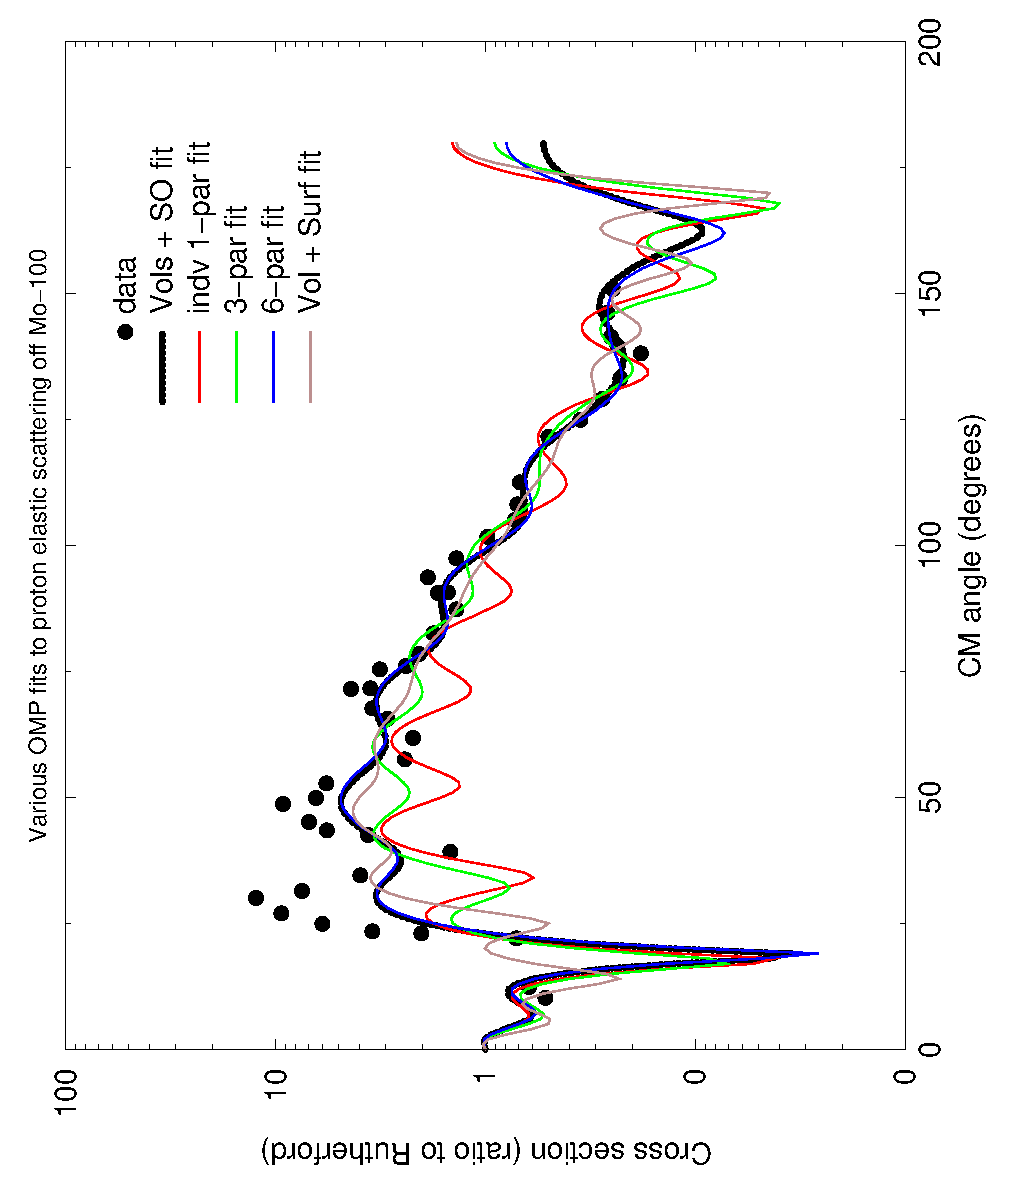
\includegraphics[width=0.78\textwidth,angle=270]{plots/SOfinal.eps}
	\caption{This plot shows how the fit changes after each stage. The red line shows the fit results after the parameters have been individually varied. The green line shows the result after the adjustments from separate 3-parameter fits of the real and imaginary volume terms are included. The blue line shows result after adjustments from the 6-parameter fit are made. The black dashed line shows the result after the spin-orbit component is included. The light brown line shows the results of fitting with real volume and imaginary surface components. The black dots are the proton elastic scattering data from \citep{Sinha1972} (error bars are smaller than the points). The adjustments made going from fitting individual parameters to sets of three and then six improve the quality of the fit. Note that inclusion of the spin-orbit component does little to improve the fit.}
	\label{fig:fits}
\end{figure}


%\begin{figure}
%\centering
%	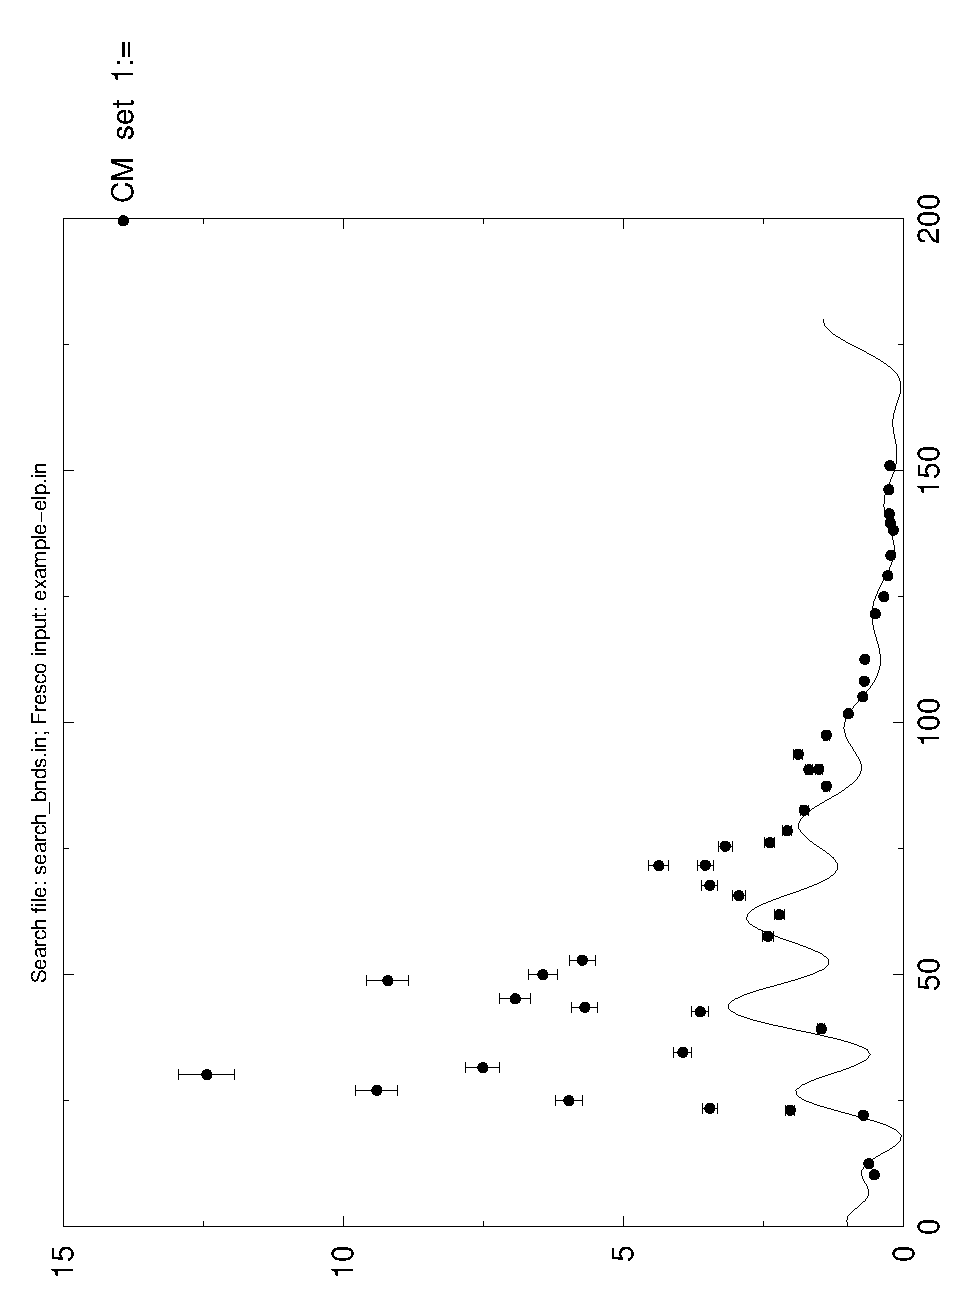
\includegraphics[width=0.78\textwidth,angle=270]{plots/searchV1.eps}
%	\caption{The result of individually fitting the six parameters of real and imaginary volume components of an OMP to the proton elastic scattering data of \citep{Sinha1972}.}
%	\label{fig:fitv1}
%\end{figure}

%\begin{figure}
%\centering
%	\includegraphics[width=0.78\textwidth,angle=270]{plots/searchV2.eps}
%	\caption{The result of iterated three-parameter fitting of real and imaginary volume components of an OMP to the proton elastic scattering data of \citep{Sinha1972}.}
%	\label{fig:fitv2}
%\end{figure}

%\begin{figure}
%\centering
%	\includegraphics[width=0.78\textwidth,angle=270]{plots/searchV3.eps}
%	\caption{The result of the iterated six-parameter fitting of real and imaginary volume components of an OMP to the proton elastic scattering data of \citep{Sinha1972}.}
%	\label{fig:fitv3}
%\end{figure}

%\begin{figure}
%\centering
%	\includegraphics[width=0.78\textwidth,angle=270]{plots/searchSOfinal.eps}
%	\caption{Fit including real and imaginary volume as well as spin-orbit components of an OMP compared to the proton elastic scattering data of \citep{Sinha1972}.}
%	\label{fig:final}
%\end{figure}


%\clearpage


%% FIT SURFACE IMAGINARY %%


%\begin{table}
%\centering
%	\begin{tabular}{ c | c c c | c c c  }
%	$E _{\mathrm{in}}$ [MeV] & $ V _0$ & $ r _0$ & $ a _0$ & $W_s$ & $ r _{ws} $ & $ a _{ws} $\\
%\hline
%	49.0 &  47.0 &  1.16 &  0.75  &  4.2 & 1.37 &  0.51\\
%\hline
%	\end{tabular}
%	\caption{Starting parameters for fitting with surface imaginary.}
%	\label{tab:initSURF}
%\end{table}

\subsection*{Real Volume and Surface Imaginary Terms}

We repeated the fitting procedure described above for an optical potential composed of a real volume term and an imaginary surface term (in place of the imaginary volume). Table~\ref{tab:fitsurf} presents our results and Figure~\ref{fig:fits} compares our fit to the data.

While neither verison of the potential fits the data particularly well, replacing the imaginary volume component with an imaginary surface worsens the fit at large CM angles ($\geq 75 ^{\circ}$). For this reason, we add the spin-orbit component to our volume-volume results. To do this, we first add the spin-orbit component (\texttt{type}$=3$) to our potential definition in the \texttt{fresco} input file. We then iterate 3-parameter fits for the real and imaginary volume parts (these are minor adjustments), then perform a 3-parameter fit on the spin-orbit parameters. Next, we perform 6-parameter fits with many combinations of parameters from the three components. Finally, we perform a full 9-parameter fit and iterate to produce our final fit (see Table~\ref{tab:fitvol} and Figure~\ref{fig:fits}). Including the spin-orbit term does not drastically improve upon the fit shown in Figure~\ref{fig:fits}.


%, however, it does shift the peaks for CM angles $\leq 50 ^{\circ}$ to better align them with the peaks in the data - at the same time disturbing the alignment of the two smaller peaks around $70 ^{\circ}$ and $100 ^{\circ}$.


\begin{table}
\centering
	\begin{tabular}{ c | c | c | c }
	Fit Type & Parameter & Value & $\chi ^2 / N$ \\
\hline
	\multirow{6}{*}{Indv. 1-par} & $a _{ws}$ & 1.49 & 258 \\
	& $r _{ws}$ & 1.18 & 226 \\
	& $a _0$ & 0.80 & 206 \\
	& $r _0$ & 1.21 & 192 \\
	& $W_s$ & 4.29 & 191 \\
	& $V$ & 47.1 & 190 \\
\hline
	\multirow{3}{*}{3-par} & $V$ & 44.2 & \multirow{3}{*}{105}\\
	& $r_0$ & 1.41 & \\
	& $a_0$ & 1.07 & \\
\hline
	\multirow{3}{*}{3-par} & $W_s$ & 4.83 & \multirow{3}{*}{104}\\
	& $r_{ws}$ & 1.26 & \\
	& $a_{ws}$ & 1.37 & \\
\hline
	\multirow{6}{*}{6-par} & $V$ & 45.3 & \multirow{6}{*}{103}\\
	& $r_0$ & 1.38 & \\
	& $a_0$ & 1.04 & \\
	& $W_{s}$ & 3.8 & \\
	& $r_{ws}$ & 1.26 & \\
	& $a_{ws}$ & 1.36 \\
\hline
	\end{tabular}
	\caption{Results fitting with a real volume and surface imaginary potential.}
	\label{tab:fitsurf}
\end{table}

%\begin{figure}
%\centering
%	\includegraphics[width=0.78\textwidth,angle=270]{plots/searchSF.eps}
%	\caption{The final fit of real volume and imaginary surface parameters to the proton elastic scattering data of \citep{Sinha1972}.}
%	\label{fig:fitsurf}
%\end{figure}



%% FIT SO %%


%\begin{table}
%\centering
%	\begin{tabular}{ c | c | c c }
%	Parameter & Value & $\chi ^2 / N$ & First Derivative\\
%\hline
%	$a _{so}$ & 1.71 & 130 & -0.81\\
%	$V_{so}$ & 8.34 & 130 & 0.12\\
%	$r _{so}$ & 1.04 & 192 & 1.1\\
%\hline
%	\end{tabular}
%	\caption{Adding a spin-orbit term to the volume real and imaginary fit results.}
%	\label{tab:fitso}
%\end{table}

%\begin{figure}
%\centering
%	\includegraphics[width=0.78\textwidth,angle=270]{plots/searchSO1.eps}
%	\caption{The final fit, adding a spin-orbit term to the real volume and imaginary terms, compared to the proton elastic scattering data of \citep{Sinha1972} ($E_{p} = 49.4$ MeV).}
%	\label{fig:fitso}
%\end{figure}

%\begin{table}
%\centering
%	\begin{tabular}{ c | c c c | c c c  }
%	$E _{\mathrm{in}}$ [MeV] & $ V _0$ & $ r _0$ & $ a _0$ & $V_{so}$ & $ r _{so} $ & $ a _{so} $\\
%\hline
%	43.8 &  43.8 &  1.16 &  0.77  &  6.0 & 1.06 &  0.78\\
%\hline
%	\end{tabular}
%	\caption{Starting parameters for adding spin-orbit to the volume (real and imaginary) fit.}
%	\label{tab:initSO}
%\end{table}




%\begin{figure}
%\centering
%	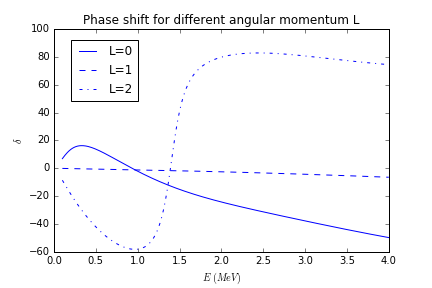
\includegraphics[width=0.85\textwidth]{figures/phase.png}
%	\caption{Phase shifts $\delta(E)$ for $l=0,1,2$. A weak resonance appears for $l=2$ near $E=1.4$ MeV with a width of $\sim 260$ keV.}
%	\label{fig:phase}
%\end{figure}

\clearpage


%%\bibliographystyle{apj}
\bibliographystyle{plain}
\bibliography{ref}

\end{document}
